\chapter{Desarrollo del Software}\label{chap:Desarrollo}

El capitulo siguiente se describirá las diferentes herramientas de software utilizadas para el desarrollo de esta tesis. El mismo se dividirá en dos secciones la primera describe los detalles técnicos como lenguaje de programación, librerías de software y entorno de trabajo; la segunda sección se muestra la organización y estructura del código realizado.


\section{Detalles Técnicos e Implementación}\label{sec:implementacion}

\subsubsection*{Python}
Python es un lenguaje de programación de código abierto y multiparadigma que permite la programación orientada a objeto, funcional e imperativa. 
Cuenta con estructuras de datos eficientes y de alto nivel, el interprete de Python puede extenderse fácilmente  con nuevas funcionalidades y tipos 
de  datos implementados en C o C++, además cuenta con una amplia comunidad de soporte y 
documentación \footnote{Fuente:www.docs.python.org.ar/tutorial}. 

Los principales motivos por el cual se optó por este lenguaje de programación es:
\begin{itemize}
 \item Facilidad de implementación y manipulación de grandes cantidades de datos.
 \item Lenguaje muy utilizado en el ámbito laboral de \ac{ml}.
 \item Posee diversas librerías para \ac{ml} y \ac{cv} en manipulación de datos e imágenes.
\end{itemize}


\subsubsection*{OpenCV}
\ac{opencv}, es una librería de código libre que nos permite manipular imágenes de manera mas eficiente; esta librería se usa en diferentes ámbitos no solo académico, sino también en ámbitos comerciales, como ejemplo en sistemas de seguridad para detección de movimiento, control de procesos, control de calidad de alimentos, automatización de vehículos y en numerosas áreas de la ciencia como robótica, detección de objetos, reconstrucciones 3D, realidad aumentada, etc. \footnote{Fuente: http://opencv.org/} La biblioteca \ac{opencv} puede ser usado bajo licencia BSD (Berkeley Software Distribution) \footnote{Fuente: https://blog.desdelinux.net/hablemos-de-la-licencia-bsd/ } para proyectos escolares o comerciales. 

\subsubsection*{Keras}

Es una interfaz de programación (API) de alto nivel para redes neuronales, escrita en python , para la manipulación y uso de modelos de \ac{cnn}. Envuelve las eficientes bibliotecas de cálculo numérico Theano y TensorFlow y permite definir y entrenar modelos de redes neuronales en unas breves líneas de código \footnote{Fuente:  https://keras.io/}. Como principal inconveniente encontrado es la escasa documentación de la librería.

\subsubsection*{Scikit-Learn}\label{sub:sklearn}
Scikit-Learn es una librería de software desarrollada en Python para solucionar problemas de \ac{ml}; que comprende en intentar predecir datos desconocidos a partir de modelos creados. Cuenta con varios algoritmos para la solución de problemas de ,regresión, clasificación y clustering, incluyendo algoritmos como maquinas de soporte vectoriales, vecino mas cercano (K-NN), descenso de gradiente , entre otros\footnote{Fuente: http://scikit-learn.org/stable/index.html}.

Su principal ventaja es la fácil implementación y manipulación de los algoritmos contenidos en la librería.

\subsubsection*{Entorno de desarrollo}
El entorno de desarrollo utilizado fue el ID \textit{Eclipse}, herramienta de código abierto multiplataforma. Esta herramienta fue diseñada para ser extendida de forma indefinida a través de \textit{plug-ins}. Sus principales características son:
\begin{itemize}
 \item Perspectivas, editores y vistas
 \item Gestión de proyectos
 \item Extensa colección de \textit{plug-ins}
\end{itemize}
El \textit{plug-ins} utilizado para el desarrollo de la tesis fue \textit{Pydev, EGit}. El principal inconveniente encontrado de esta herramienta es 
el consumo de memoria en ejecución, así también se presentaron inconvenientes a la hora de realizar integración en entornos colaborativos como Git.

\subsubsection*{Control de Versiones}

Las herramientas que se utilizaron para llevar un control del versiones en el desarrollo fueron: \textit{GitHub}\footnote{Fuente: https://github.com/} y \textit{GitLab} \footnote{Fuente : https://about.gitlab.com/} , son software pensado en el mantenimiento de aplicaciones. El objetivo de estas aplicaciones gestionar los diversos cambios que se realizaron sobre los elementos de algún producto o alguna configuración del mismo; una versión, revisión o edición del producto, es el estado en el cual se encuentra el mismo.

Las características principales son: herramientas gráficas para ver como se trabajo en el proyecto, entorno colaborativo permitiendo a diferentes desarrolladores compartir sus trabajos, registro histórico de cada acción realizada en cada elemento, seguimiento de errores.

\subsubsection*{ENVI}\label{sub:enviSoft}

El software de análisis de imágenes \textit{ENVI} es utilizado por profesionales de GIS, científicos e analistas de imágenes para extraer información significativa de las imágenes para tomar mejores decisiones. ENVI se puede implementar y acceder desde el escritorio, en la nube y en dispositivos móviles y puede personalizarse a través de una API para cumplir con los requisitos específicos del proyecto \footnote{Fuente: http://www.harrisgeospatial.com/Learn.aspx}.

ENVI proporciona una poderosa API que permite agregar sus propios algoritmos propietarios, ampliar las herramientas y modelos existentes, automatizar las tareas de alta frecuencia y combinar múltiples herramientas para producir los resultados deseados.

El principal inconveniente encontrado es la instalación de herramientas adicionales para la manipulación de las imágenes como,\textit{ VIIRS Toolkit}. Otra falencia encontrada es lo poco amigable para el usuario a la hora de trabajar con imágenes.

\section{Organización y Estructura del código}\label{sec:estructuracodigo}

La organización del código experimental se dispuso en varios componentes separados con el fin de hacer el código mas re-utilizable.

La estructura del directorio de trabajo es la siguiente:
\begin{itemize}
 \item \textbf{CNN}: Las funciones que contiene realizan el calculo del \textit{feature vector} a través de una red neuronal utilizando la librería 
\textit{Keras}.
 \item \textbf{ImgManipulation}: Almacena las diferentes funciones que permiten la manipulación de las imágenes de entrada 
 \item \textbf{Notacion}: Contiene diferentes clases que permiten calcular los bounding box y \ac{nms}; también contiene las funciones que almacenan 
la notaciones.
 \item \textbf{Proposal}: Contiene la clase que ejecuta regions proposal.
 \item \textbf{TensorF}:Almacena las funciones que permiten realizar el entrenamiento de los datos utilizando \textit{Scikit-Learn}.
\end{itemize}

\begin{figure}[H]
 \centering
  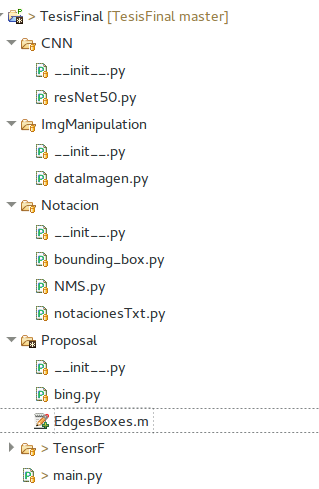
\includegraphics[height=10cm,keepaspectratio=true,clip=true]{imagenes/Logos/structureData.png}
  \caption{Estructura de directorio de trabajo}
\end{figure}


\textbf{main.py}\\
Este scripts constituye la parte principal del proceso automatizado; llamando a las diferentes clases mencionadas previamente. Las principales 
acciones que lleva a cabo son:
\begin{itemize}
 \item Lee las carpetas que contiene las imágenes junto con las anotaciones de cada una de ellas.
 \item Comprueba que exista las notaciones
 \item A cada imagen realiza el crop(recorte) correspondiente.
 \item Extrae las anotaciones de cada imagen.
 \item Llama a la clase para calcular \textit{regions proposal}.
 \item Calcula el \textit{overlapping}, \ac{nms} para cada imagen.
 \item Calcula los \textit{features vectors}
 \item Almacena los datos en un archivo .mat
 \item Para finalizar realiza una llamada a la función para el entrenamiento.
\end{itemize}

\subsubsection*{Documentación}\label{sub:documentacion}
Para documentar el desarrollo realizado se utilizo la herramienta \textbf{\textit{Doxygen}}. Esta herramienta es un generador de documentación de fácil integración y uso en python.